\documentclass[11pt,a4paper]{article}
\usepackage[T1]{fontenc}
\usepackage[margin=2.3cm]{geometry}
\usepackage{amsmath,amssymb}
\usepackage{graphicx}
\usepackage[dvipsnames]{xcolor}
\usepackage{enumitem}
\usepackage[colorlinks=true,linkcolor=blue,urlcolor=blue]{hyperref}
\setlength{\parskip}{0.6em}
\setlength{\parindent}{0pt}
\begin{document}

\begin{center}{\LARGE\bfseries openkymo}\\[0.4em]{\large Turn a video into one picture and read speed off its stripes, in three sessions.}\\[0.2em]\small PAN IIT OSS explainer \textbullet{} higher secondary to advanced undergraduate (levels 4-6)\end{center}

\section*{Why this exists}
A video is a stack of pictures, which is a lot of data for one question: how fast does it move? This explainer shows how keeping one line of pixels from every frame turns a video into a single picture whose stripe slopes are speeds, and how to measure those slopes honestly.

\section*{The end goal}
Read flow speed off the stripe slopes of a kymograph. The end goal is to read flow speed off the stripe slopes of a kymograph, the technique used to measure convection speeds in flames, blood and cell transport, drops, belts and many other flows. The same idea is also a first step towards optical flow and motion tracking.

\section*{How the three sessions build up}
\begin{enumerate}[nosep]
\item \textbf{Session 1: One line of pixels, stacked over time} (Level 1, conceptual interactive model, 60 min).
\item \textbf{Session 2: Slope to metres per second, and how fast the camera must be} (Level 2, mathematical engineering model, 75 min).
\item \textbf{Session 3: Synthetic kymographs: measure, break and validate} (Level 3, simulation and validation, 90 min).
\end{enumerate}

\section{Session 1: One line of pixels, stacked over time}

\subsection*{A. Real-world problem}
A bead rolls along a tube, a drop falls past a window, a bright patch rides on a flame. A video shows that things move, but a video is hard to measure: thousands of frames, each one a full picture. What if you kept only one line of pixels from each frame and stacked those lines into a single image? Then a whole video becomes one picture, and the speed becomes something you can read with a ruler: the slope of a stripe.

\subsection*{B. Concept and theory}
A video is a stack of frames. Each frame is a grid of brightness numbers. Choose one row of the grid (the line) and cut that row out of every frame. Stack the cut-out rows with frame 0 at the top: you get a new image called a kymograph. Its columns are positions along the line (pixels) and its rows are time (frames). If a bright blob sits at pixel x0 in frame 0 and moves v pixels in every frame, it is at x0 + v t in frame t, so in the kymograph it draws a straight stripe. The slope of that stripe, dx/dt, is the speed v in pixels per frame. A still object has v = 0 and makes a vertical stripe. A faster object makes a stripe that is tilted further from vertical. Section B of Session 2 turns pixels per frame into metres per second.

\begin{itemize}[nosep]
\item t: frame number (time, counted from 0) (frames)
\item x: position along the chosen line (pixels)
\item x0: blob position in frame 0 (pixels)
\item v: speed of the blob = slope of the stripe dx/dt (pixels per frame)
\item K(t, x): kymograph brightness at row t and column x (brightness units)
\end{itemize}

\begin{equation*}
x(t)=x_0+v\,t
\end{equation*}

\begin{equation*}
v=\frac{x_2-x_1}{t_2-t_1}=\frac{\Delta x}{\Delta t}
\end{equation*}

\begin{equation*}
K(t,x)=\text{frame}_t[\text{row},\,x]
\end{equation*}

\begin{center}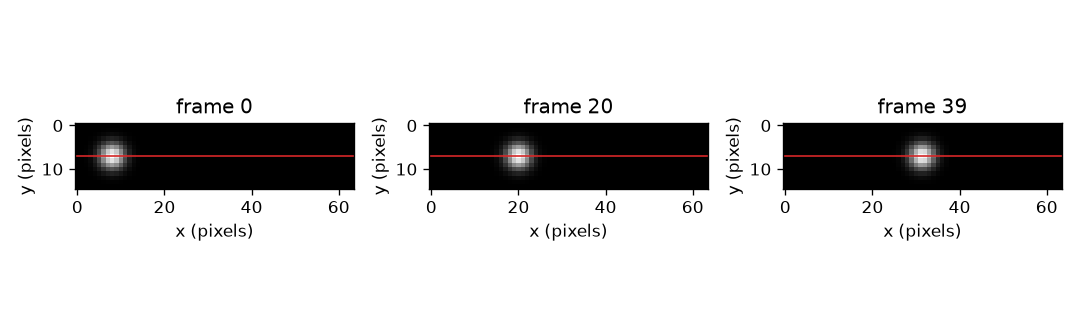
\includegraphics[width=0.85\linewidth]{figures/s01_frames_and_line.png}\\\small Three frames of a tiny video; the red line is the row that is stacked into the kymograph.\end{center}

\subsection*{E. Worked example}
In the video of Figure 1 the blob moves at 0.6 px/frame from x0 = 8. Find its column in frames 10 and 30 and the slope between them.
\begin{enumerate}[nosep]
\item Position in frame 10: 8 + 0.6 * 10 = 14.
\item Position in frame 30: 8 + 0.6 * 30 = 26.
\item Slope = (26 - 14) / (30 - 10) = 12 / 20 = 0.6 px/frame.
\item Sanity check: over 39 frames the blob moves 0.6 * 39 = 23.4 pixels, from 8 to 31.4, well inside the 64 pixel line.
\end{enumerate}
\textbf{Answer.} The blob is at column 14 in frame 10 and column 26 in frame 30; the stripe slope is 0.6 px/frame.

\subsection*{F. Questions}
\begin{enumerate}[nosep]
\item \textbf{Conceptual.} What does a vertical stripe mean? What would a bright horizontal stripe (the same row lit up in a single frame) mean?
\item \textbf{Numerical.} A blob is at column 5 in frame 0 and at column 41 in frame 30. Find its speed in px/frame and check that it stays on a 64 pixel line for 40 frames.
\item \textbf{Graph and simulation interpretation.} In the app, how does the stripe look in the kymograph and how does the line look in the position graph when you triple the speed from 0.3 to 0.9? Which picture shows the faster object as steeper?
\item \textbf{Design and optimisation challenge.} Design: the line is 64 pixels long, the blob starts at pixel 8, and you want it to stay on the line for at least 30 frames while you measure. Which speeds are allowed? Why would a very slow blob also be a poor choice?
\end{enumerate}

\section{Session 2: Slope to metres per second, and how fast the camera must be}

\subsection*{A. Real-world problem}
An engineer asks: how fast does the air move in this flame, or how fast is the belt going? A slope of 0.8 pixels per frame is not an answer. We need the size of a pixel on the real object, the number of frames per second, and a way to measure the slope using every pixel of the stripe, not two hand-picked points. And before filming, we must choose the camera settings so that the measurement can work at all.

\subsection*{B. Concept and theory}
A pattern that moves rigidly has brightness K(t, x) = f(x - v t). Differentiating gives Kt + v Kx = 0, where Kx is the brightness change per pixel and Kt per frame. Every pixel gives one such equation. The structure tensor J collects the sums of Kx Kx, Kx Kt and Kt Kt over the whole image into a 2x2 matrix. Its eigenvector for the larger eigenvalue (nx, nt) is the direction in which brightness changes fastest, which is across the stripes. The stripes run perpendicular to it, so v = -nt / nx. The coherence (big minus small eigenvalue over their sum) is close to 1 when the stripes are clean and parallel. In real units: one pixel covers a size dx on the object (millimetres, divided by 1000 for metres) and the camera takes fps frames each second, so speed in m/s = slope * dx * fps. The method assumes the pattern moves only a small fraction of its own width between frames. A safe rule for a blob is a shift per frame of at most 0.5 pixel (and never above 1 pixel). The shift per frame is v / (dx fps), so the slowest allowed frame rate is fps\_min = v / (0.5 dx), and the line must be at least shift * n\_frames pixels long to hold a stripe for n\_frames frames.

\begin{itemize}[nosep]
\item v\_px: stripe slope (pixels per frame)
\item dx: size of one pixel on the object (mm per pixel, divided by 1000 for m) (mm/px)
\item fps: frame rate of the camera (frames per second)
\item v: speed of the object (m/s)
\item Kx, Kt: brightness change per pixel and per frame (brightness units per pixel, per frame)
\item J: structure tensor, 2x2 matrix of summed products of gradients (brightness units squared)
\item nx, nt: components of the main eigenvector of J (no unit)
\item shift: pixels moved between two frames = v\_px (pixels per frame)
\end{itemize}

\begin{equation*}
K(t,x)=f(x-vt)\;\Rightarrow\;K_t+v\,K_x=0
\end{equation*}

\begin{equation*}
J=\begin{pmatrix}\sum K_xK_x & \sum K_xK_t\\ \sum K_xK_t & \sum K_tK_t\end{pmatrix},\qquad v=-\frac{n_t}{n_x}
\end{equation*}

\begin{equation*}
v_{\mathrm{m/s}}=v_{\mathrm{px}}\cdot\frac{\mathrm{mm/px}}{1000}\cdot \mathrm{fps}
\end{equation*}

\begin{equation*}
\tan\varphi=v_{\mathrm{px}},\qquad \mathrm{shift}=\frac{v}{(\mathrm{mm/px}/1000)\,\mathrm{fps}}\le 0.5\;\Rightarrow\;\mathrm{fps}\ge\frac{v}{0.5\,(\mathrm{mm/px}/1000)}
\end{equation*}

\begin{center}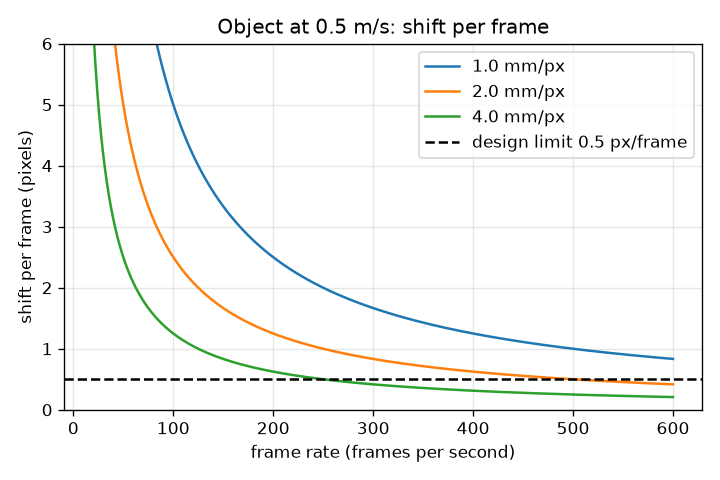
\includegraphics[width=0.85\linewidth]{figures/s02_shift_vs_fps.png}\\\small Shift per frame against frame rate for an object at 0.5 m/s with three pixel sizes; the dashed line is the 0.5 px/frame design limit.\end{center}

\subsection*{E. Worked example}
A stripe has the slope 0.8 px/frame. The camera records 200 fps and one pixel covers 1.5 mm. Find the speed in m/s and the angle of the stripe from the time axis.
\begin{enumerate}[nosep]
\item Pixel size in metres: 1.5 mm / 1000 = 0.0015 m.
\item Speed = 0.8 px/frame * 0.0015 m/px * 200 frames/s = 0.24 m/s.
\item Angle = arctan(0.8) = 38.7 degrees from the time axis (45 degrees would be 1 px/frame).
\item Unit check: (px/frame) * (m/px) * (frames/s) = m/s.
\end{enumerate}
\textbf{Answer.} The object moves at 0.24 m/s; the stripe is tilted 38.7 degrees from the time axis.

\subsection*{F. Questions}
\begin{enumerate}[nosep]
\item \textbf{Conceptual.} Why does the stripe direction equal the direction perpendicular to the main eigenvector, and why is v = -nt / nx with a minus sign?
\item \textbf{Numerical.} A stripe has slope 0.45 px/frame, the pixels are 0.8 mm wide and the camera runs at 500 fps. Find the speed in m/s and check the units.
\item \textbf{Graph and simulation interpretation.} On the shift-per-frame graph for 0.5 m/s, at what frame rate does the 2 mm/px curve reach 0.5 px/frame, and what about the 4 mm/px curve? What does a coarser pixel buy you, and what does it cost?
\item \textbf{Design and optimisation challenge.} Design: a camera is fixed at 240 fps and the object moves at 0.8 m/s. What is the smallest pixel size (mm/px) that keeps the shift at 0.5 px/frame or less? How long must the line be to hold the stripe for 40 frames at that shift? State the trade-off.
\end{enumerate}

\section{Session 3: Synthetic kymographs: measure, break and validate}

\subsection*{A. Real-world problem}
Before you trust a method on a real video you must test it where the answer is known. You build kymographs with a given speed, add noise and measure. Then you ask the engineer's questions: how wrong is the answer when the picture is noisy? At what speed does the method stop working? And when a conveyor belt is filmed with too few frames per second, can we still believe the number the program prints?

\subsection*{B. Concept and theory}
A synthetic kymograph with known speed is the numerical experiment: it is the trusted reference. Estimator 1 uses the gradients. The least-squares (LS) form v = -sum(Kx Kt) / sum(Kx Kx) assumes Kx is exact; noise in Kx makes the denominator too big and pulls the answer towards zero. The total least squares (TLS) form takes the main eigenvector of the structure tensor of Session 2, built from derivative-of-Gaussian images, where the noise in Kx and Kt is equal and independent and only adds the same amount to both diagonal entries, so the eigenvector, and v, are not biased. Estimator 2 follows one stripe: in each row it takes the brightness-weighted centre within a window around the last position, then fits x = x0 + v t by least squares. For n equally spaced points with scatter sigma\_x about the line, the standard deviation of the fitted slope is sigma\_x * sqrt(12 / (n (n\textasciicircum{}2 - 1))). Aliasing: if a pattern repeats every wavelength lambda pixels and moves d pixels per frame, frames cannot tell d from d minus k lambda, so the camera reports d folded into the range minus lambda/2 to plus lambda/2. A single smooth blob survives larger shifts than the 1 pixel rule suggests (to about 3 px/frame for a blob of width 1.5 px), but once the shift is a few times the blob width, neighbouring frames no longer overlap and the gradient equation Kt + v Kx = 0 no longer holds.

\begin{itemize}[nosep]
\item K(t, x): kymograph brightness (brightness units)
\item sigma: blob width (standard deviation of the Gaussian) (pixels)
\item noise: standard deviation of the noise added to every pixel (brightness units (blob height = 1))
\item sigma\_x: scatter of the tracked centres about the fitted line (pixels)
\item n: number of points (frames) in the line fit (no unit)
\item lambda: wavelength of a periodic pattern (pixels)
\item d: true shift between two frames (pixels per frame)
\end{itemize}

\begin{equation*}
v_{\mathrm{LS}}=-\frac{\sum K_xK_t}{\sum K_xK_x}
\end{equation*}

\begin{equation*}
\sigma_{v}=\sigma_x\sqrt{\frac{12}{n\,(n^2-1)}}
\end{equation*}

\begin{equation*}
d_{\mathrm{app}}=\left[(d+\lambda/2)\bmod\lambda\right]-\lambda/2
\end{equation*}

\begin{equation*}
\text{relative error}=\frac{\hat v-v}{v}
\end{equation*}

\begin{center}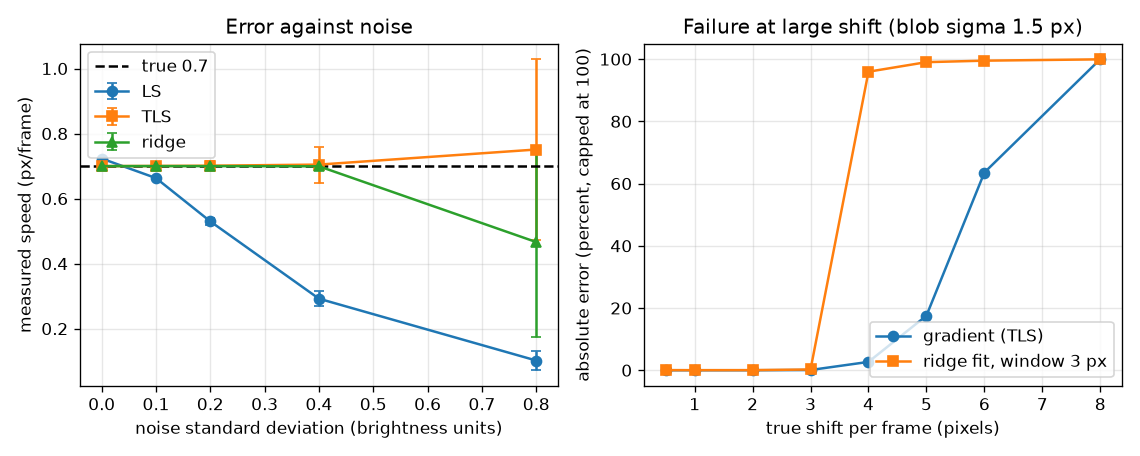
\includegraphics[width=0.85\linewidth]{figures/s03_error_study.png}\\\small Left: measured speed against noise for LS, TLS and the ridge fit. Right: error against shift per frame for the blob.\end{center}

\subsection*{E. Worked example}
A cosine pattern of wavelength 8 px moves 5 px/frame to the right. What shift does the camera report, and what is the standard deviation of a slope fitted through 60 tracked points with scatter 0.26 px?
\begin{enumerate}[nosep]
\item Apparent shift = 5 folded into -4 .. +4: 5 - 8 = -3 px/frame. The pattern seems to move backwards at 3 px/frame.
\item Check by the program: the gradient estimator on this synthetic pattern reports -2.94, within 0.1 of -3.
\item Slope scatter = 0.26 * sqrt(12 / (60 * (60\textasciicircum{}2 - 1))) = 0.26 * sqrt(12 / 215 940) = 0.26 * 0.00745 = 0.0019 px/frame.
\item Simulation with 2000 noisy fits gives 0.0019 as well.
\end{enumerate}
\textbf{Answer.} The camera reports -3 px/frame (backwards); the fitted slope scatter is 0.0019 px/frame.

\subsection*{F. Questions}
\begin{enumerate}[nosep]
\item \textbf{Conceptual.} Why does noise bias the least-squares speed towards zero, and why does the total least-squares (structure tensor) speed not suffer from this bias?
\item \textbf{Numerical.} A ridge tracker gives 40 centre points with scatter 0.3 px about the fitted line. What is the standard deviation of the fitted slope in px/frame, and how large is it relative to a true speed of 0.5 px/frame?
\item \textbf{Graph and simulation interpretation.} In the right panel of the error figure, up to which shift per frame are both methods exact for this blob (width 1.5 px), what happens first, and which method fails first?
\item \textbf{Design and optimisation challenge.} Design: a belt moves at 0.8 m/s and each pixel covers 2 mm. From the conveyor experiment (worst error over 5 seeds: 18.5 percent at 100 fps, at most 0.2 percent from 200 fps up) choose a frame rate for production. Justify it and say what you give up.
\end{enumerate}

\section{Real-world mini-project}
\textbf{Measure the speed of a conveyor belt from a kymograph.} A camera looks along a conveyor belt with a speckled surface. The belt really moves at 0.80 m/s and one camera pixel covers 2 mm. Use \texttt{conveyor\_kymo} and \texttt{belt\_speed\_mps} from Session 3 to find the smallest frame rate in the list 100, 200, 300, 400, 600, 800 frames per second for which the measured speed is within 2 percent of the truth for every one of 5 different noise seeds (seeds 0 to 4).

\section{The path ahead}
\begin{enumerate}[nosep]
\item \textbf{Session 4: Moving versus static stripes.} A function that separates the moving stripes from the static ones before measuring.
\item \textbf{Session 5: Stripes in both directions.} An estimator that returns every dominant velocity, not only one.
\item \textbf{Session 6: Beat the noise.} A line-integral (Radon or shear-sum) speed estimator and its Monte Carlo study.
\item \textbf{Session 7: Unwrap an aliased speed.} A routine that uses two sub-sampled versions of the same data to find the true shift.
\item \textbf{Session 8: A falling drop: speed along a curved stripe.} A function that returns the local speed at every frame without hand-picked windows.
\end{enumerate}

\section{Answers and hints}

\subsection*{Session 1}
\begin{enumerate}[nosep]
\item \textbf{Conceptual.} Hint: Time runs down the picture and position runs across. Solution: A vertical stripe stays at the same column in every frame, so the object does not move. A horizontal stripe lies in one row only, i.e. in a single frame, and covers many columns: the whole line lit up at the same moment, such as a flash of light or an object so fast that it crosses the whole line within one frame. It is not a sign of a moving object that can be measured.
\item \textbf{Numerical.} Hint: Speed = change in position divided by change in frame number. Solution: Speed = (41 - 5) / 30 = 1.2 px/frame. In 40 frames it travels 1.2 * 40 = 48 pixels, from 5 to 53, which is inside 64 pixels, so it stays on the line. Unit: pixels per frame.
\item \textbf{Graph and simulation interpretation.} Hint: Compare which axis is time in each picture. Solution: In the position graph time is the horizontal axis, so tripling the speed triples the slope: a steeper line (0.9 against 0.3 pixels per frame). In the kymograph time runs downwards, so the stripe becomes flatter, further tilted from vertical: it covers three times as many columns for each row. Same motion, different axes.
\item \textbf{Design and optimisation challenge.} Hint: The blob must still be on the line at frame 30, so 8 + 30 v is below the last pixel; think about how many pixels of motion a slope fit has to work with. Solution: Stay below pixel 56 (leave a margin of about 7 pixels) at frame 30: 8 + 30 v \textless{}= 56 gives v \textless{}= 1.6 px/frame. A very slow blob, say 0.05 px/frame, moves only 1.5 pixels in 30 frames, less than a blob width, so the slope is hard to read against pixel rounding. A useful range is about 0.2 to 1.6 px/frame. Trade-off: a faster blob uses the line up sooner, a slower one gives a less accurate slope.
\end{enumerate}

\subsection*{Session 2}
\begin{enumerate}[nosep]
\item \textbf{Conceptual.} Hint: Brightness is constant along the stripe and changes fastest across it. Write the gradient of f(x - v t). Solution: Along a stripe the brightness does not change, so the gradient (the direction of fastest change) points across the stripe, perpendicular to it. For K = f(x - v t) the gradient is f' * (1, -v), so (nx, nt) is proportional to (1, -v) and v = -nt / nx. The minus sign comes from -v t in the argument: a pattern moving right (v \textgreater{} 0) has a gradient that tilts to negative nt.
\item \textbf{Numerical.} Hint: Convert millimetres to metres first. Solution: 0.8 mm = 0.0008 m. Speed = 0.45 * 0.0008 * 500 = 0.18 m/s. Unit check: (px/frame)(m/px)(frame/s) = m/s. Sanity: 0.45 px/frame is less than 0.5, so the design rule is met.
\item \textbf{Graph and simulation interpretation.} Hint: Solve v / (dx * fps) = 0.5 for fps. Solution: For 2 mm/px: fps = 0.5 / (0.5 * 0.002) = 500 fps. For 4 mm/px: fps = 0.5 / (0.5 * 0.004) = 250 fps. A coarser pixel halves the frame rate needed because the object moves fewer pixels between frames. The cost is spatial detail: the pattern must still be several pixels wide, so small features are lost.
\item \textbf{Design and optimisation challenge.} Hint: Rearrange shift = v / (dx fps) \textless{}= 0.5 for dx. Solution: dx \textgreater{}= v / (0.5 * fps) = 0.8 / (0.5 * 240) = 0.00667 m = 6.67 mm per pixel (zoom out or use binning). A shift of 0.5 px/frame over 40 frames needs 0.5 * 40 = 20 pixels of line. Trade-off: coarser pixels (6.67 mm) lose detail, so the moving pattern must be larger than a few pixels (about 2 cm or more); a faster camera would allow finer pixels but needs more light and storage.
\end{enumerate}

\subsection*{Session 3}
\begin{enumerate}[nosep]
\item \textbf{Conceptual.} Hint: Where does noise enter in the formula, and what does equal noise in Kx and Kt do to the matrix J? Solution: In LS the noise adds to sum(Kx Kx) in the denominator but averages out in sum(Kx Kt), so the ratio shrinks and the speed is pulled towards zero (for a true 0.7: 0.723 with no noise, 0.530 at noise 0.2, 0.102 at noise 0.8). With equal independent noise in Kx and Kt, J gets the same amount added to both diagonal entries (J + c I), which changes the eigenvalues but not the eigenvectors, so v = -nt/nx is unchanged. The price: scatter grows with noise (0.278 at noise 0.8).
\item \textbf{Numerical.} Hint: Use sigma\_x * sqrt(12 / (n (n\textasciicircum{}2 - 1))) with n = 40. Solution: sigma\_v = 0.3 * sqrt(12 / (40 * 1599)) = 0.3 * sqrt(1.876e-4) = 0.3 * 0.0137 = 0.0041 px/frame, i.e. 0.8 percent of 0.5. Sanity: more points would give a smaller scatter, roughly as n to the power minus 3/2.
\item \textbf{Graph and simulation interpretation.} Hint: Compare the errors in the printed table at 3, 4, 5 and 6 px/frame. Solution: Both are within 0.2 percent up to 3 px/frame. At 4 px/frame the ridge tracker with a 3 pixel window loses the blob (error -96 percent) while the gradient method is still within 2.7 percent. The gradient method degrades from 5 px/frame (17.5 percent) and is 63.6 percent off at 6 px/frame. So the ridge tracker (limited by its window) fails first. The gradient method works much beyond the 1 pixel per frame rule for a smooth blob, but the rule remains the safe design value for sharp features.
\item \textbf{Design and optimisation challenge.} Hint: Compare the smallest passing rate (error below 2 percent) with the rules of Session 2 and keep a safety margin. Solution: 200 fps passes (2 px/frame, error 0.1 percent) but sits just below the failing region (4 px/frame fails with 18.5 percent), so the margin is thin and depends on this speckle size. A production choice is 400 fps (1 px/frame, the hard limit of Session 2) or 800 fps (0.5 px/frame, the design rule). Cost: more light is needed for short exposures, and more data to store and process. Assumption: the speckle and noise level of the test; a real belt with finer texture would fail earlier.
\end{enumerate}

\section{How to join}
Read \texttt{CONTRIBUTING.md} in the repository, then pick an issue labelled \texttt{good first issue}. Repository: \url{https://github.com/KrunalPanchal1995/openkymo}

\end{document}
